\section{The Prototype}

This section describes the technical details regards to our implementation. We first outline the language and framework this prototype is developed on, then we describe the rendering, layout, and orientation calculation. Lastly we go over the configuration files, events, timed and randomized sequences, and integrated questionaries that aid us in user-experimentation.

Note: Since this project is not mainly focused on the usability study of this concept, we only implemented the minimum-viable-product to carry-out the user experiments due to time-constraints. We discuss how this prototype could be improved in future>prototype section.

\subsection{Platform}

The prototype is mostly developed in Processing \cite{RN103} (a Java-based graphic-centric language mostly used in education, prototype, and visual arts) and Unity Engine (a popular free-to-use game engine). The Unity engine wraps around the Processing prototype to provide user-testing interface such as integrated questionaries and videos.

We chose Processing and Unity as they have strong support of 3D environment, video and audio playback, robust mouse input, ease-of-use, and quick prototype turn-around overheads. Both frameworks are also cross-platform and can execute on Windows, macOS, and Linux. However, as we also discuss in Section limitations section, recent macOS update added a *Gatekeeper* security feature that prevents un-sighed software from running\cite{RN105} --- thus complicating the user-testing process, as distributed prototype executables to the participants cannot be opened.

\subsection{3D Environment}\label{section:3denv}

\begin{figure}
	\centering
 	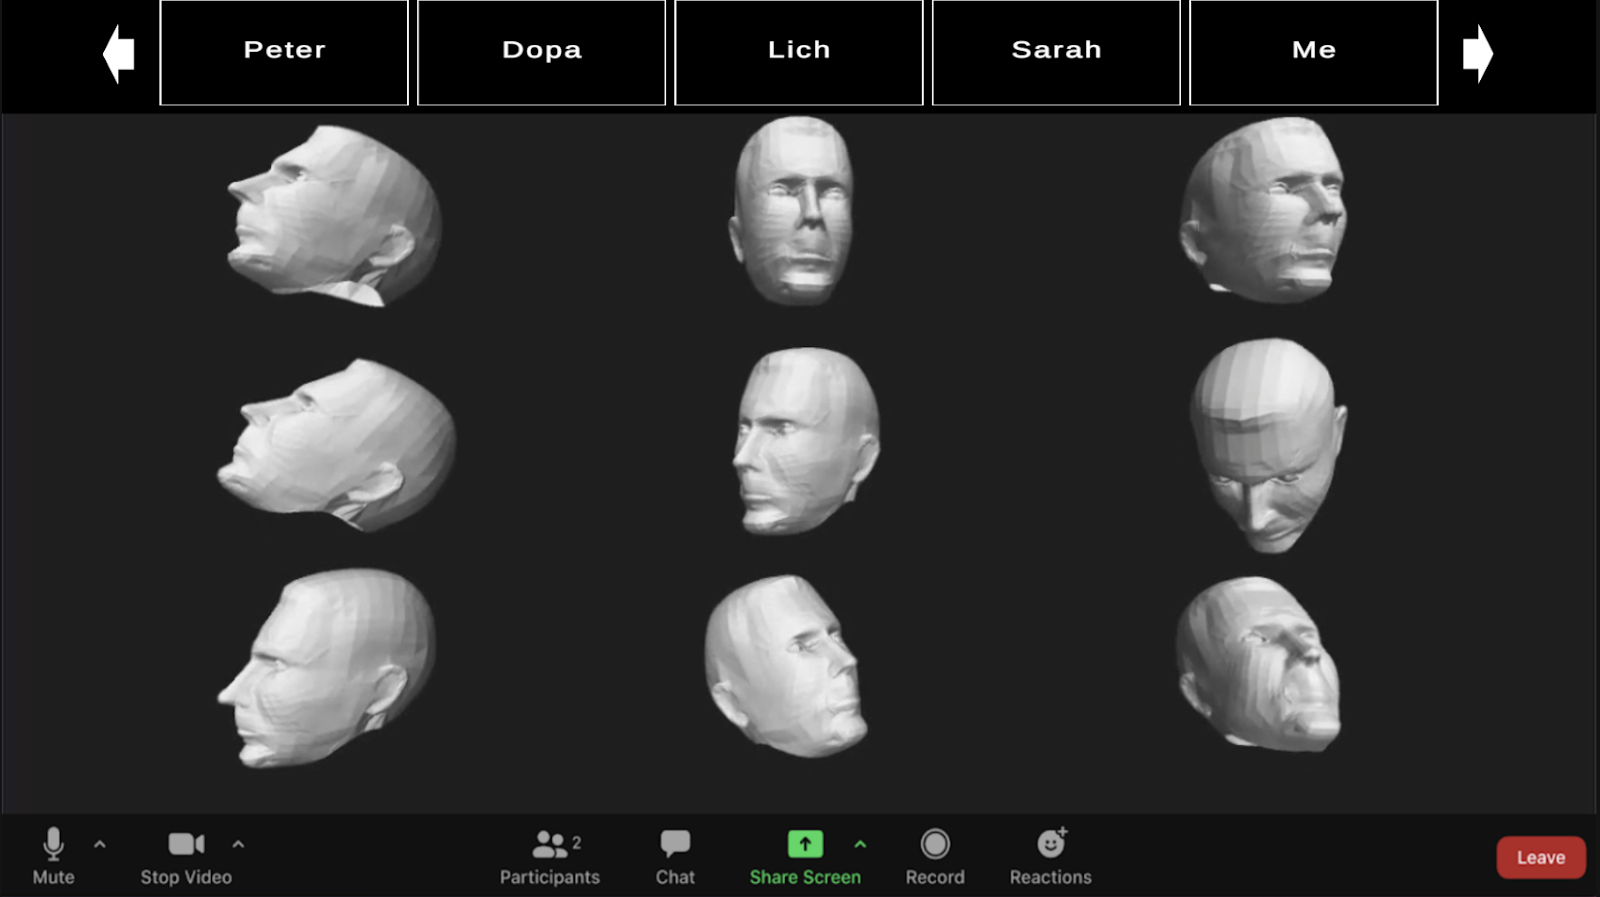
\includegraphics[width=0.9\textwidth]{unity.PNG}
	\caption{A typical view of the FutureGazer prototype app with the Unity interface}
	\label{fig:unity}
\end{figure}

Figure \ref{fig:unity} shows a typical 3D environment rendered in the prototype app. We base the user interface (UI) design --- including colours, buttons, and layout --- from existing WVC apps such as Zoom to present the participants with a familiar user experience. By doing so, we limit other factors that would interfere with our user experiments. However unlike traditional WVC apps, we replace the centre (where typically there would be a gallery or grid view of camera video feeds) with our prototype avatar representation.

From hereafter, we will refer to these visual representation of participants in the meeting as \textit{Avatar Views}. As outlined earlier in \ref{section:rq}, we propose two types of avatars to explore: 3D head avatars and 2D eye avatars. 

\begin{figure}
    \centering
    \begin{subfigure}[b]{0.4\textwidth}
        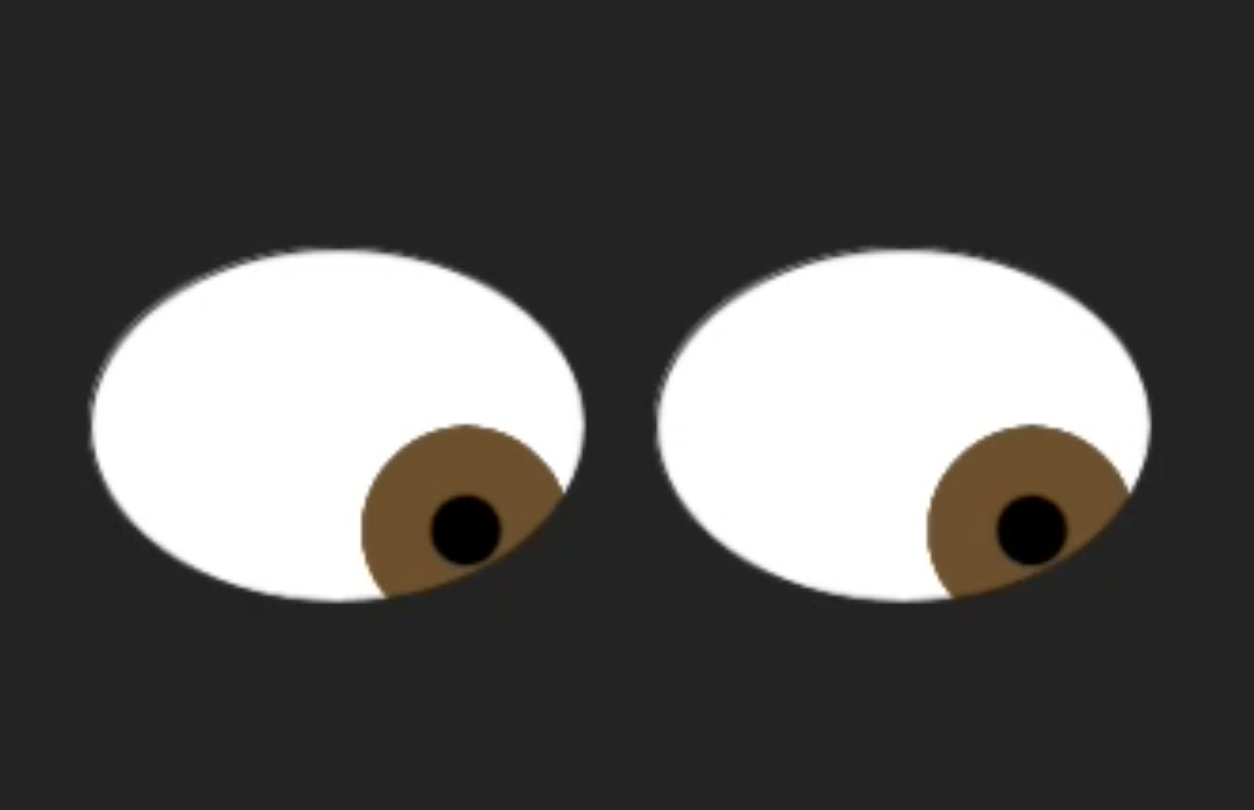
\includegraphics[width=\textwidth]{eyes.png}
        \caption{2D eyes avatar}
        \label{fig:eyes}
    \end{subfigure}
    ~
    \begin{subfigure}[b]{0.4\textwidth}
        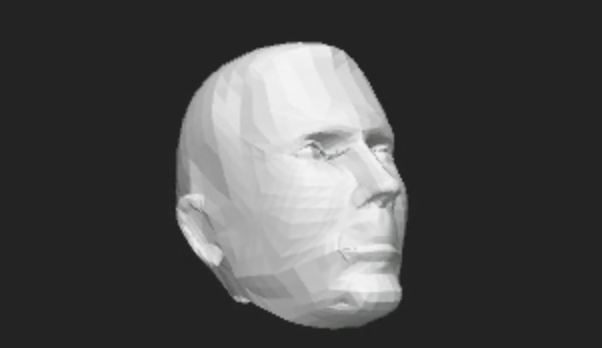
\includegraphics[width=\textwidth]{head.png}
        \caption{3D head avatar}
        \label{fig:head}
    \end{subfigure}
    \caption{2D eyes and 3D heads are the two types of avatars in FutureGazer prototype}
\end{figure}

For user experiments, we create \textit{mock avatars} to replicate/simulate real meeting participants. This creates an illusion for the test participants as if they’re real people to help us speed up the testing process without involving lots of people. However, as it is an illusion, it might affect how people perceive our prototype --- as we discuss in Section \ref{section:lim}.


\subsubsection{Heads}

\begin{figure}
	\centering
 	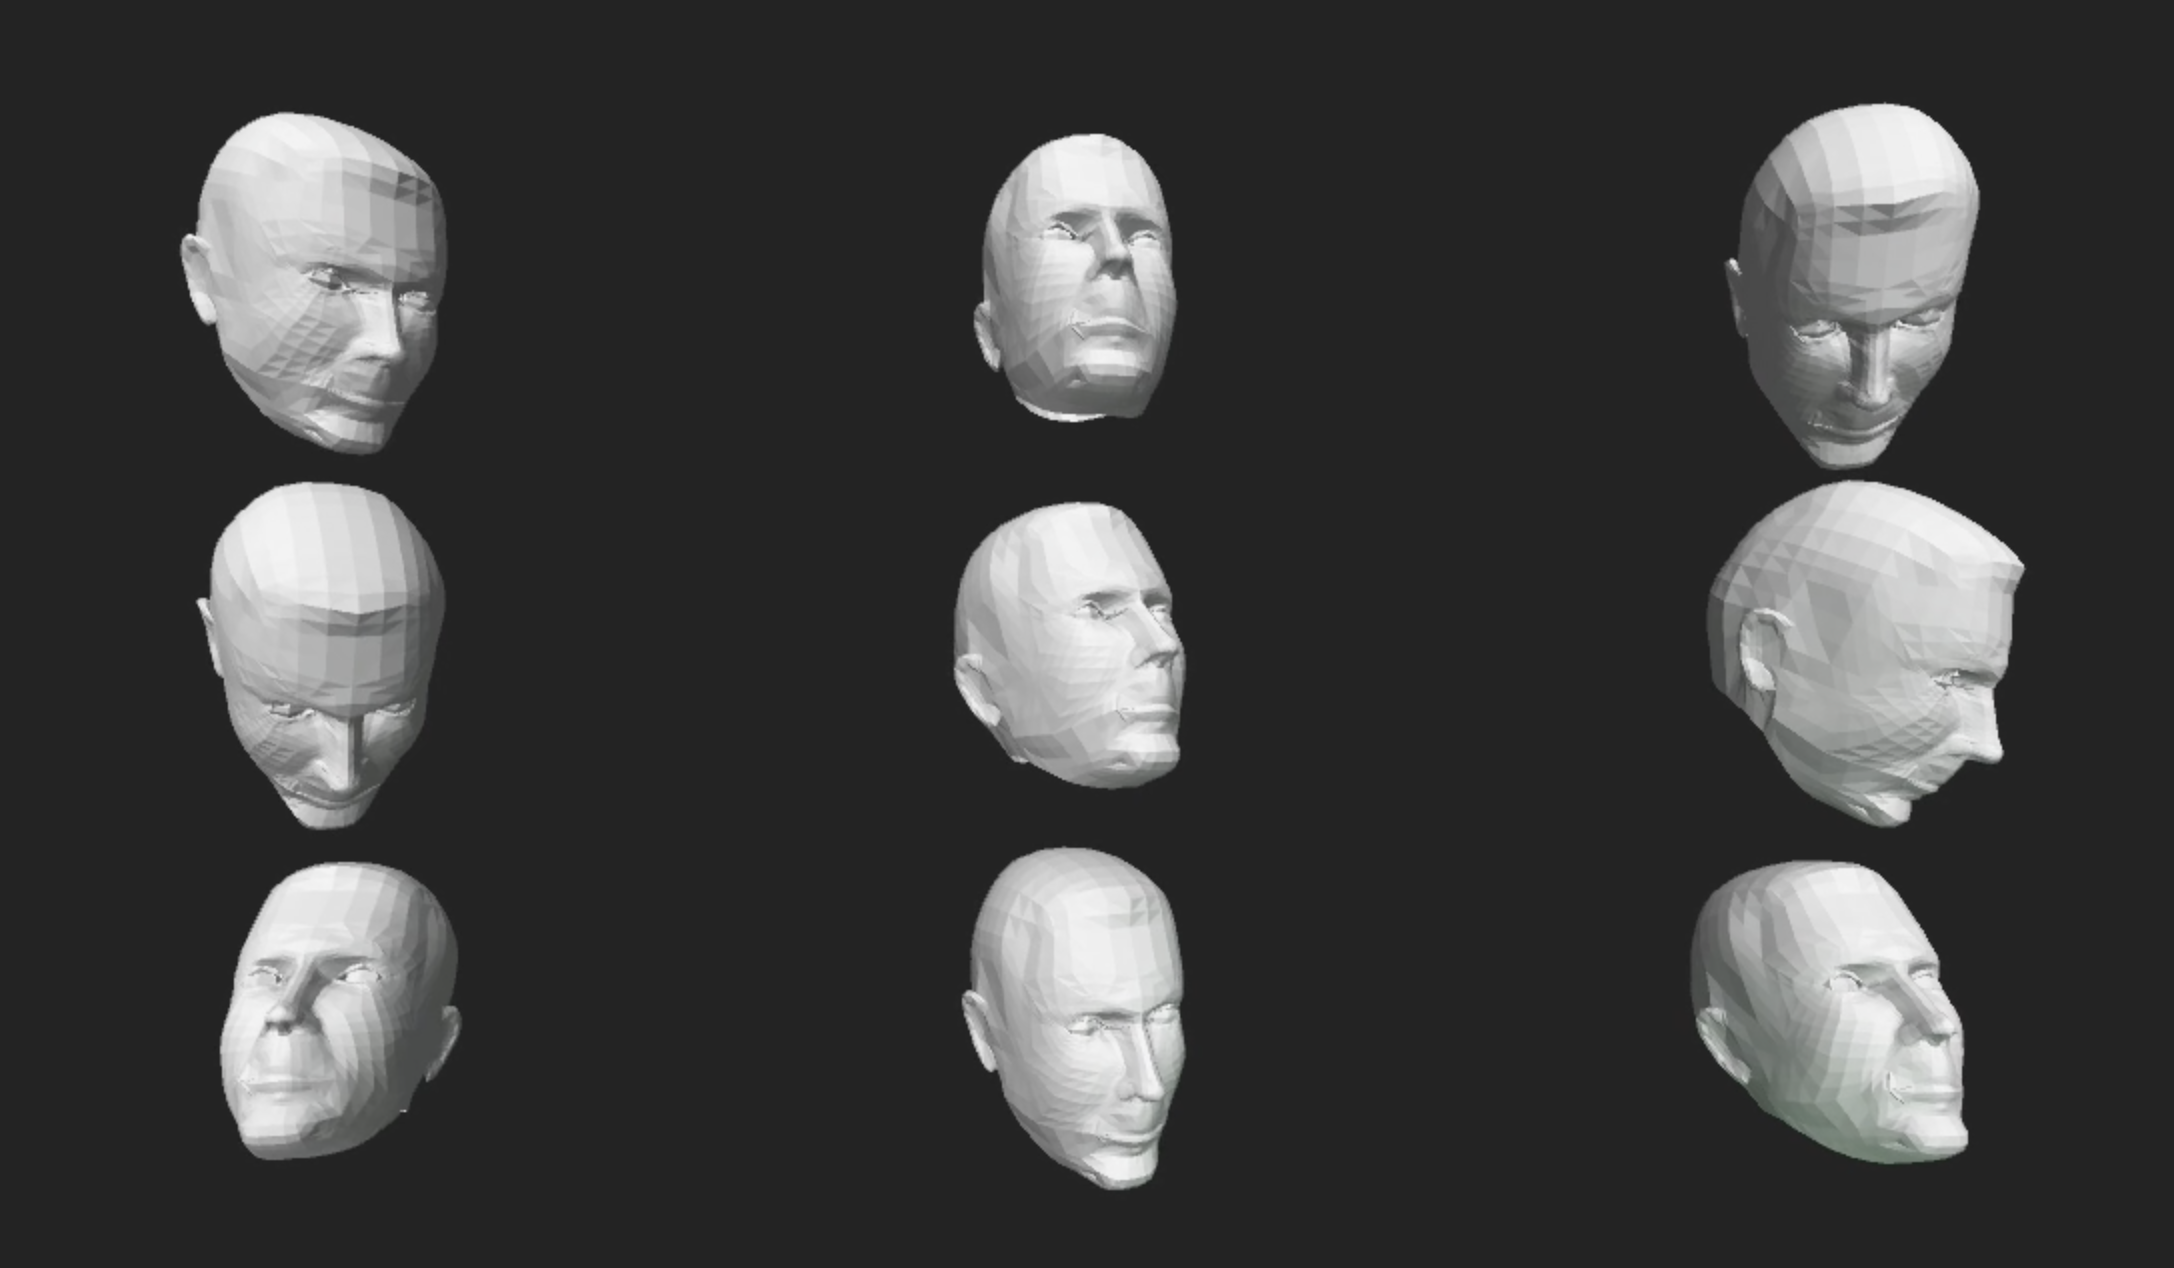
\includegraphics[width=0.9\textwidth]{headgrid.png}
	\caption{Nine head avatars fitted inside a grid view}
	\label{fig:headgrid}
\end{figure}

In the 3D environment, the head avatars are loaded from a free-to-use .OBJ 3D model downloaded from \textit{TurboSquid} with standard usage license \cite{RN104}. 
We load the object into the 3D scene once, and use the same model instance for all other head avatar objects to save computation --- since they’re essentially the same 3D model, just redrawn with different transformations.

Due to time and budget constraints, we are limited to a low-polygon-count model of the head, with no texture, no rigging, no soft-body animation, and no physics simulation. The 3D model of the head, as shown in Figure \ref{fig:head}, has minimum features of a face. Despite the low-quality 3D models, the primitiveness of the 3D model helps maintaining a high rendering frame-rate while the prototype is running, even without writing custom shaders and performing fine-tuned optimizations --- especially when there could potentially be up to 9 to 25 avatars being drawn concurrently on to the screen. This is important as we need the head avatars to transform and render in real-time as if they’re real inputs in a WVC application.
As we will discuss in Section \ref{section:lim}, if given more budget and 3D talent, more work can be allocated to polishing the visual appeal of the avatars to be more inviting and friendly, and ultimately improve user-experience.

\subsubsection{Eyes}

The 2D eyes avatar was inspired from goggly eyes and novel desktop widgets (e.g. XEyes\cite{RN50}) created as general amusement. However, we decided to explore this as an alternative to the head avatars to see whether if 3D and head orientation is required to deliver eye-contact and gaze hints to the meeting participants. 

\begin{figure}
	\centering
 	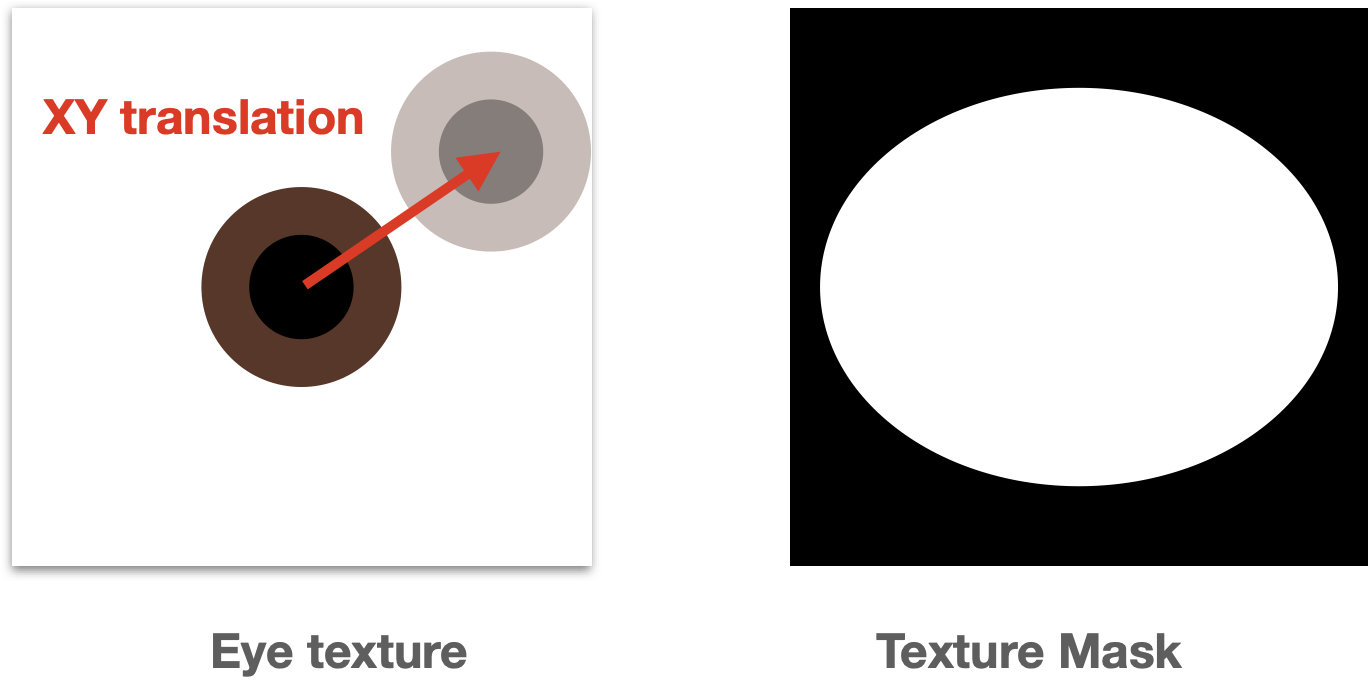
\includegraphics[width=0.5\textwidth]{eyebreakdown.png}
	\caption{Breakdown of how an eye is rendered for eye avatars}
	\label{fig:eyebreakdown}
\end{figure}

insert eye avatar view

insert eye avatar grid view

With eyes avatars, instead of a 3D object transformed to orient a direction, we simply render a pair of pupils and irises on a white background as a sub-image/texture (Figure \ref{fig:eyebreakdown}). Then depending on where the eye should be looking at, we rendering this sub-image with a transform that translates it in $x$ or $y$ direction (Figure \ref{fig:eyebreakdown}). Finally, we create an eye mask that only only renders the eye itself (Figure \ref{fig:eyebreakdown}).

The result is somewhat similar to a gallery view of meeting participants in a traditional WVC application, except with only the eyes and their gaze visually represented.

\subsubsection{UI Elements}

As discussed in Section \ref{section:3denv}, the 3D head avatars and 2D eye avatars are rendered at $z=0$. In front of that, we render the UI elements such as the bottom menu bar, as well nameplates to aid in our experiments and to provide a familiar environment to the participants.

\begin{figure}
	\centering
	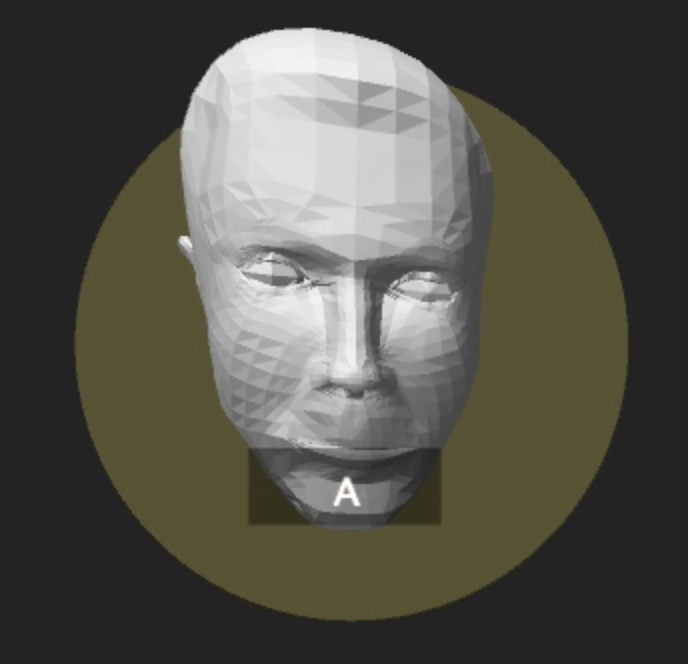
\includegraphics[width=0.5\textwidth]{halo.png}
	\caption{A Halo highlights avatars that are in focus, i.e. whoever is talking}
	\label{fig:halo}
\end{figure}

\begin{figure}
	\centering
	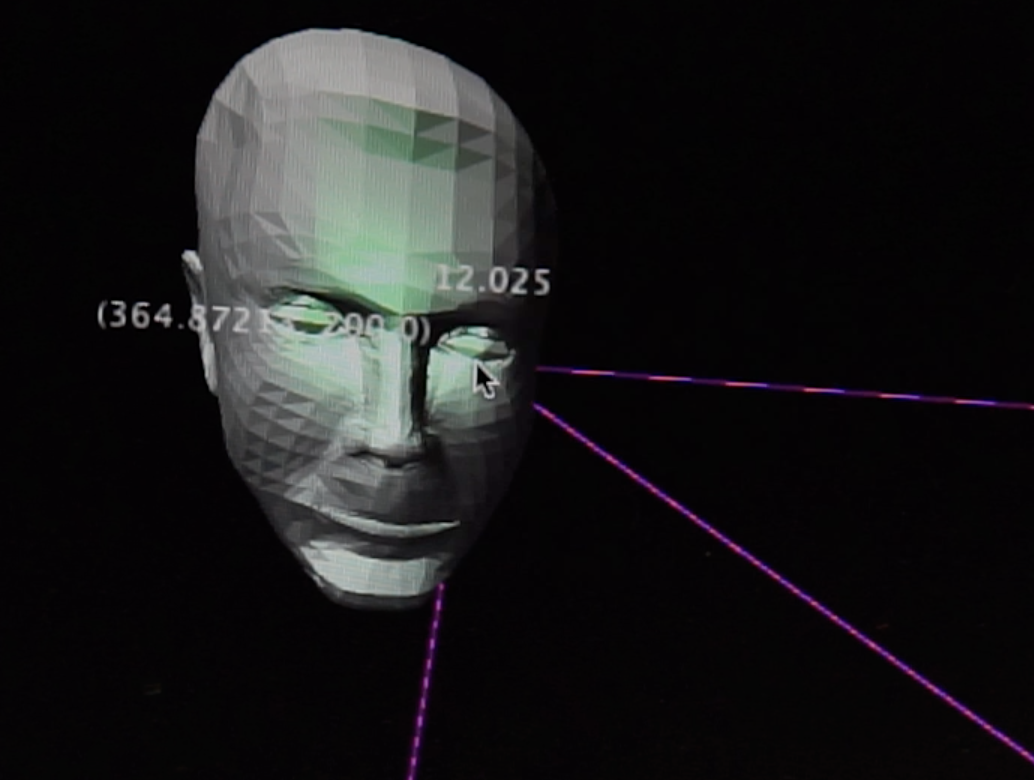
\includegraphics[width=0.5\textwidth]{pointlight.png}
	\caption{Point light highlights where the mouse is}
	\label{fig:pointlight}
\end{figure}

In Figure \ref{fig:halo}, when a participant corresponding to an avatar is talking, we have an option to activate a yellow halo behind the avatar for indication. To do this, each avatar base class has a flag \texttt{isFocused} that can be toggled. If this flag is on, then we draw this additional halo on a layer behind the avatars.

While not used in our final experiments, we also added an option to highlight avatars in on the screen based on mouse cursor positions. Rather than drawing a bounding box around the avatar, we thought it was appropriate to instead model the mouse cursor effects as a point-source-light with some vibrant colour, such as seen in Figure \ref{fig:pointlight}. This option can be turned on via experiment configuration file (see Section \ref{section:config}). 

\subsection{View Modes}

To simplify the behaviour of mock avatars, we have three pre-programmed modes for the avatars to follow:

\begin{enumerate}
    \item \textbf{NORMAL}: the avatar is in normal mode, it will follow and track a given set of target coordinates (see Section \ref{section:target-coord}).
    \item \textbf{STARE}: the avatar should stare at the active participant by gazing directly outwards from the screen.
    \item \textbf{RANDOM}: the avatar randomly looks around as if they are distracted. Current implementation of the random mode uses a series of Perlin noise functions to approximate how real head moves around randomly.
\end{enumerate}

Note that this would only apply to the mock avatars used in user experiments to simulate real people.

During user experiments, we can dynamically and programmatically change the modes of the avatars to simulate whether a person in the meeting is paying attention or not paying attention, and looking at the test subject participant, or anywhere else on the screen.


\subsection{View Calculation}

This section talks about the math and algorithms created to compute the target coordinates --- the screen-space coordinates of where that avatar should be looking at. As well as the mapping between the target coordinates to a rotation (for head avatars) or a translation (for eye avatars) transformations.

\subsubsection{Target Coordinates}\label{section:target-coord}

Each avatar (*View* base class) has attributes targetX and targetY which corresponds to where the avatar should directly look at in *normal* mode. These attributes are not used in *random* and *stare* modes.

For example, if the avatar is set to track the mouse cursor’s screen position, then we trivially set:

\begin{lstlisting}[language=Java]
avatar.targetX = mouseX
avatar.targetY = mouseY
\end{lstlisting}


If an avatar A is set to look at another avatar B, we can set the target coordinates of A to the spatial coordinates of B:

\begin{lstlisting}[language=Java]
A.targetX = B.x
A.targetY = B.y
\end{lstlisting}

\subsubsection{Rotation Calculation}

Once an avatar knows \textit{where} to look (i.e. the target coordinates),
it needs to compute \textit{how} to look in that direction (i.e. compute the corresponding transforms required to show the correct visual representation).

% insert image of mapping from targetXy to offset Xy

For the 2D eye avatars, this mapping from target coordinates to transformation is a simple 2D translation $(\Delta x, \Delta y)$, as seen in Figure \ref{fig:eyebreakdown}. First, a difference vector $\vec d$ is computed from the avatar’s local origin to the target coordinates. We then scale it by some factor $s$ to control the sensitivity of this translation. Finally, we constrain the magnitude of $s\vec d$ to the radius of the eyes to ensure the pupil do not go off the eye, creating a white eye.

For the 3D head avatars, the mapping is instead from the target coordinates to a set of rotations along the x, y, and z-axis. The simplest way to do this is to draw a 3D vector from the head avatar origin to the target coordinates. Then using trigonometry on the vector, we can find all angles corresponds to the x, y, and z rotations.

Notice, that up to this point, we have not established the third, z-component, of the target coordinates. This is because it depends on what the head avatar should be looking at. If the avatar is looking at another avatar, we leave $z = 0$ since all avatars are on the $z = 0$ plane. However, if the avatar were to follow the mouse or stare at the user, then we must set $z = z^\prime$, where $z^\prime$ is the z-offset of the camera. The difference between with vs. Without this z-correction can be seen in Figure \ref{fig:rot-correct}.

% insert figure of heads looking straight on vs at the camera

\begin{figure}
    \centering
    \begin{subfigure}[b]{0.6\textwidth}
        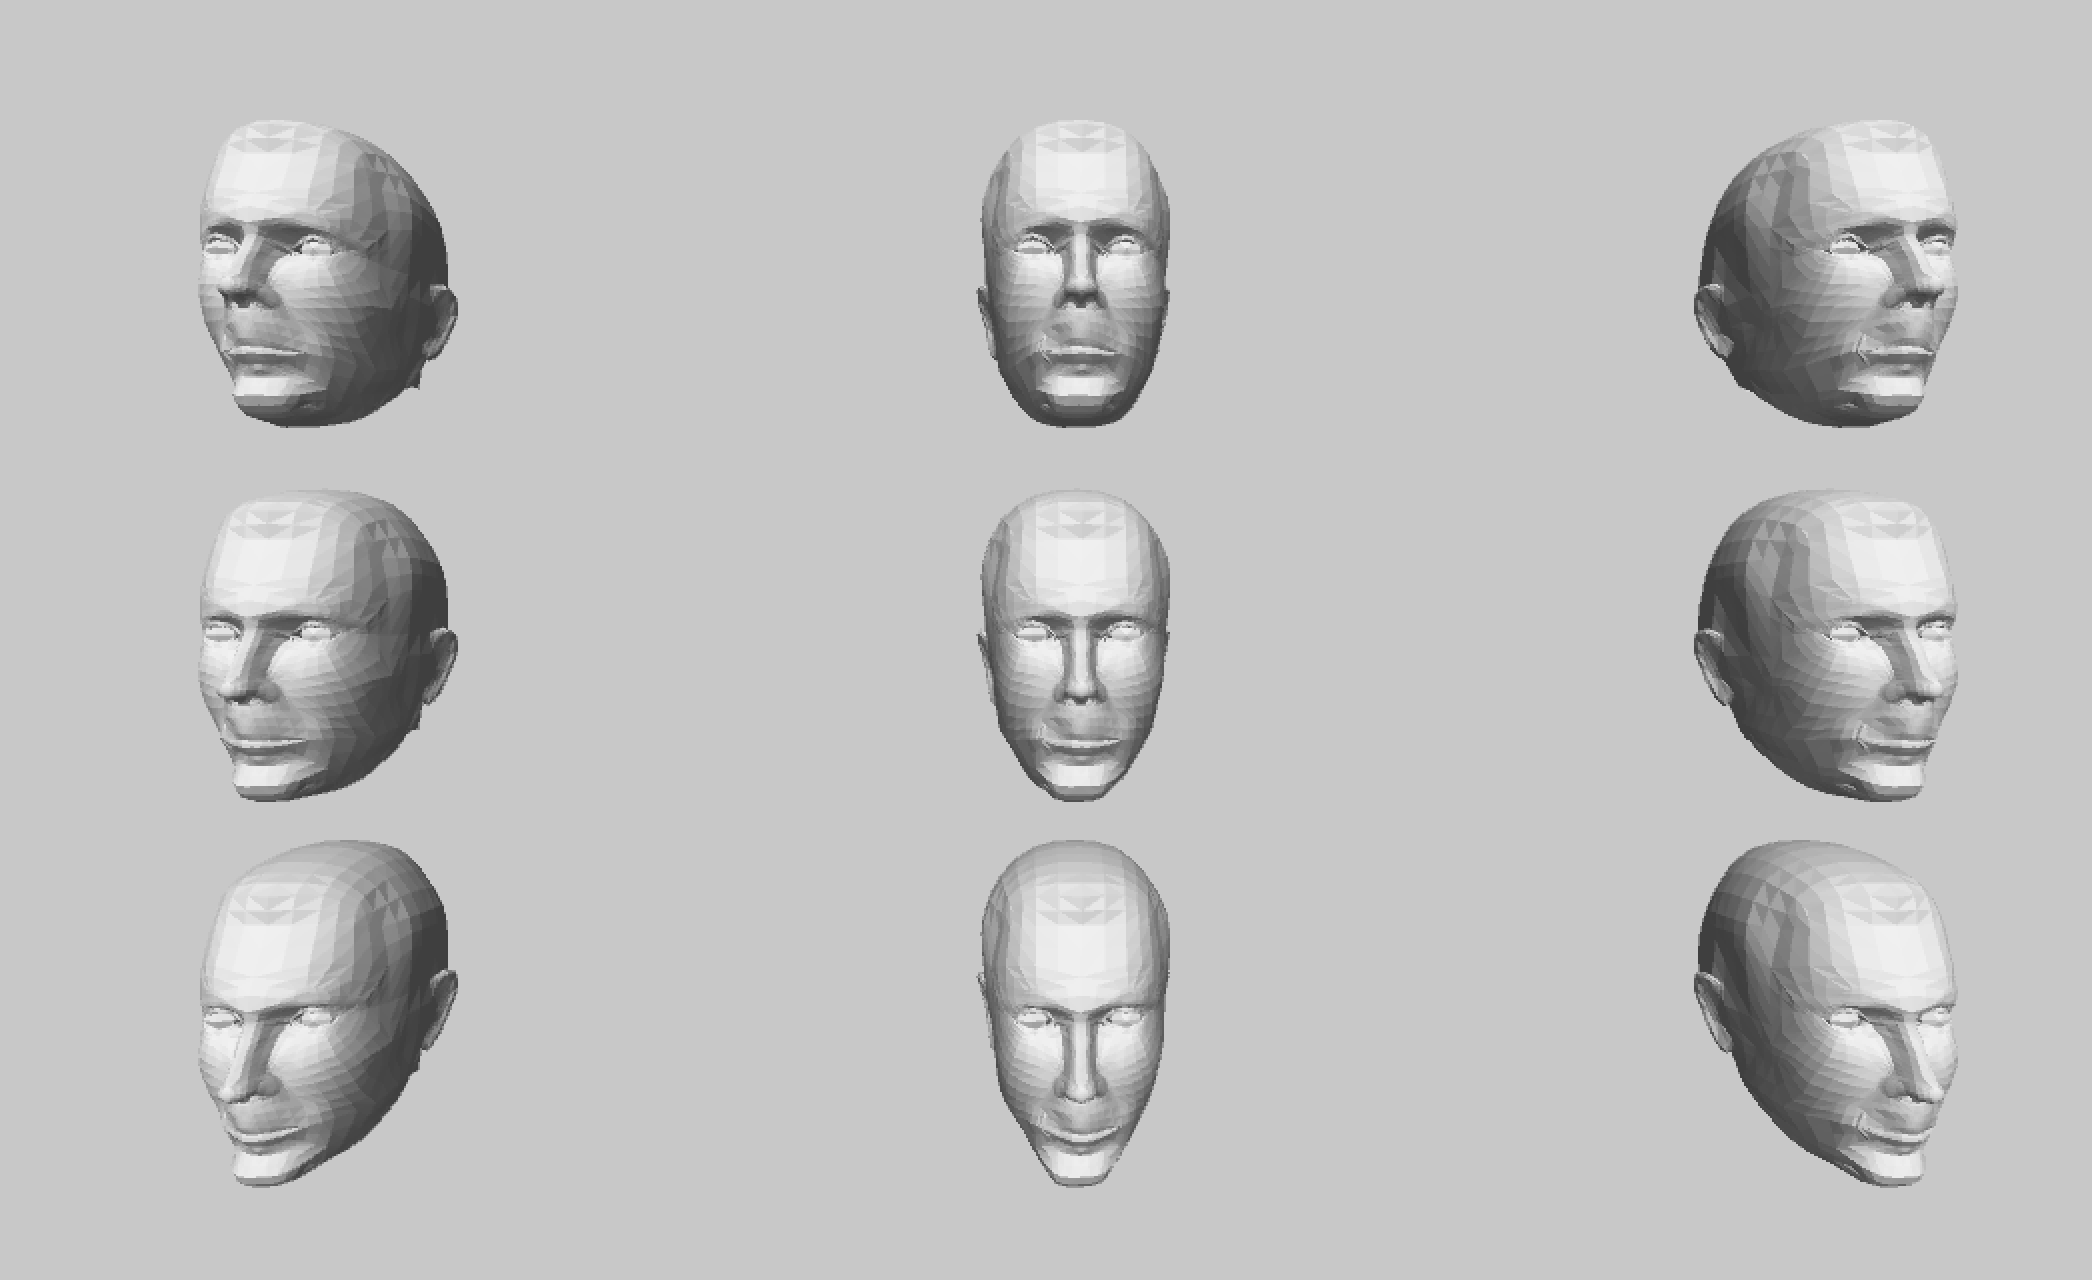
\includegraphics[width=\textwidth]{grid-nocorrect.png}
        \caption{A grid of head avatars without rotation offset correction}
    \end{subfigure}
    ~
    \begin{subfigure}[b]{0.6\textwidth}
        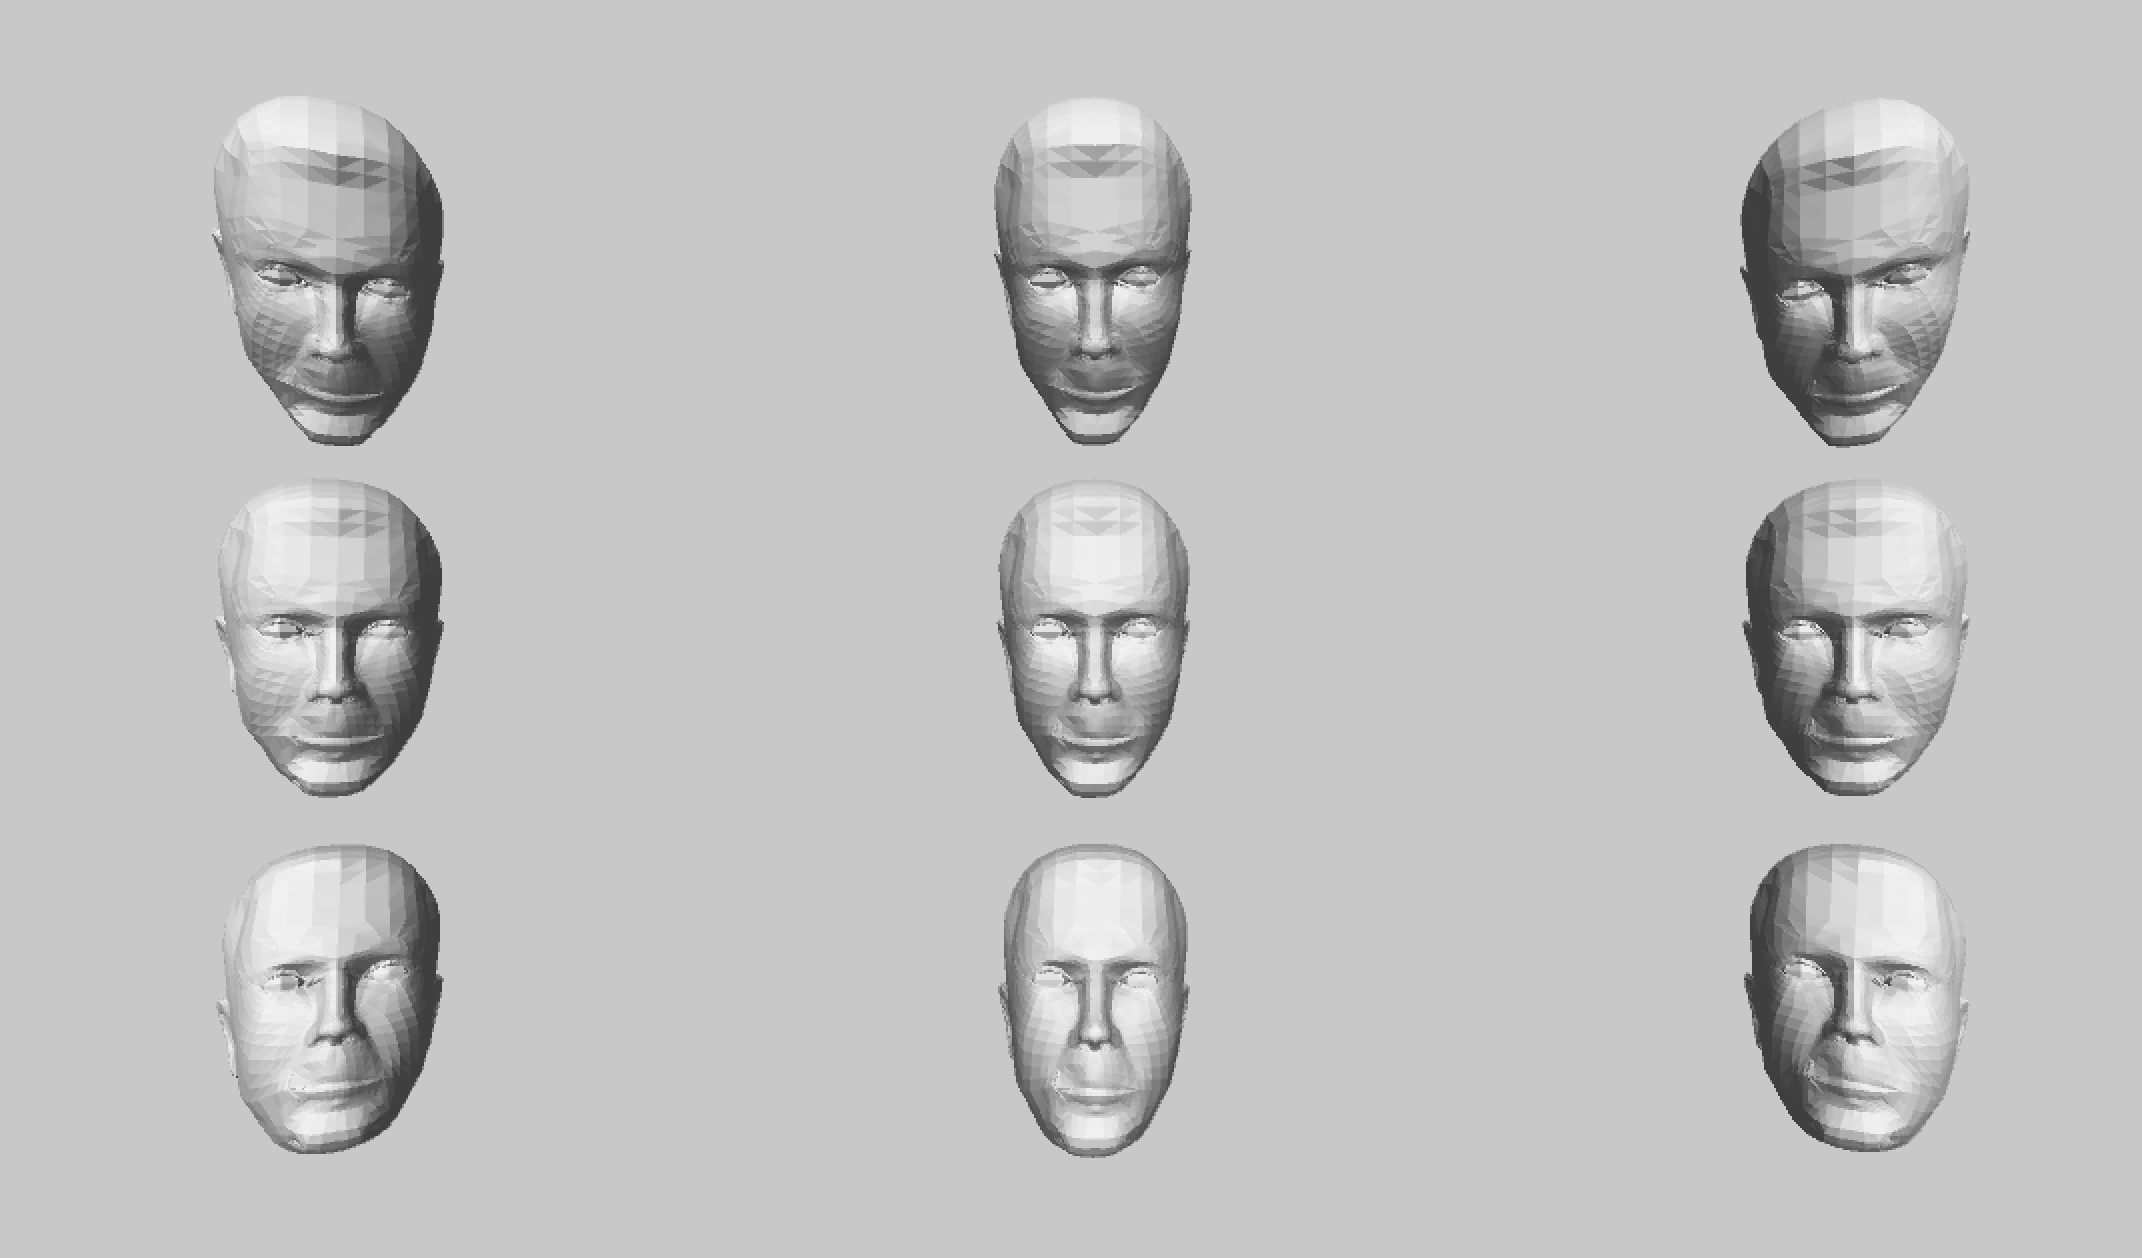
\includegraphics[width=\textwidth]{grid-correct.png}
        \caption{A grid of head avatars with rotation offset correction}
    \end{subfigure}
    \caption{Grid of heads require some rotation offset to stare out of the screen}
    \label{fig:rot-correct}
\end{figure}

\subsubsection{Realism Approximations}

For both eye and head avatars, instead of applying the transformation in the renders according to he target coordinates instantaneously, we use a linear-interpolation function to smoothen the motion and simulate a more natural response --- a response with mass, inertia, and a sense of reaction time delay that would exist in real people.

We also added an option to make the head wobble controlled by some noise to make the avatars feel less robotic and more organic. If a 3D head avatar’s isFocused flag is set on (such as when the participant the avatar belongs to is speaking), the wobble amplitude is slightly increased to approximate the extra motion due to mouth movements.

\subsection{Configuration Files}\label{section:config}

To facilitate a series of automated, consistent, yet randomly generated user experiment scenarios, we developed a configuration framework for our prototype. Each experiment setup (see Section \ref{section:exp}) is contained inside a config.json file. Each file contains all the experiment parameters such as number of avatars, type of avatars, names, and the sequence of modes, target coordinates, etc. 

\subsubsection{Initialization}

The file can be loaded at initialization-time of the experiment. Upon which, all the parameters in the configuration file is read, and the defined avatars are populated in the scene. 

\subsubsection{Events}

The sequence of state changes in the prototype user experiment is controlled by *events*. These events are defined in the configuration files as a single array that represents a timeline. The different types of events supported are:

\begin{itemize}
    \item Change mode
    \item Change avatar target
    \item Set focus flags
    \item Play sound
    \item Stop experiment
\end{itemize}

For more details regarding events, please refer to the source code.

\subsection{Unity Engine Wrapper}

To further facilitate user testing, we wrapped the Processing prototype in a Unity engine user interface, where participants are guided without the constant supervision from us. Each experiment setup is sequenced in order and appropriate questionaries are prompted in between each setup. Finally, the questionnaire responses are automatically logged in participants’ computer, making it easy for review.
